\chapter{Author Extraction}\label{cha:author-extraction}

In this chapter, we will discuss author extraction as a concrete use case for the usage of \glspl{crf} in combination with \gls{distant supervision}.
This can be broken down into to following steps:
\begin{enumerate}
  \item Preprocessing of research papers to extract reference sections as text from \gls{pdf} documents
  \item Generating tagged training sets for distant supervision
  \item Building \gls{ge} constraints
  \item Learning a \gls{crf} model using \gls{ge} constraints
\end{enumerate}
The following sections will describe these steps in more detail.
In addition, we will formulate a number of research questions that we aim to answer in \Cref{cha:evaluation}.
These research questions will focus on the use case of extracting authors from research papers in the area of German social sciences.
We will also highlight some of the similarities and differences of our approach to the one of \citet{lu2013web}.

\section{Preprocessing}\label{sec:ae-preprocessing}

Before building a training set using \gls{distant supervision}, an unlabeled training data set needs to be generated.

Since we want to learn a model that is able to extract author names in reference sections, it is crucial to remove the text that is not part of the reference section.
Otherwise, we would also match names that appear in the body of the research paper during the author name matching step (see \Cref{subsec:ae-author-name-matching}).
In order to incorporate the layout of the research paper, this step of detecting reference sections ideally should be performed before converting the \gls{pdf} document into a textual format.
This would for example allow an accurate detection of headers or page numbers.

\bigskip

Either before or after detecting reference sections, the textual content of the research paper has to be extracted.
For this, the layout of the document needs to be recognized in order to correctly extract the text from a research paper.
For example, research papers can contain two columns of text per page.
Without considering the layout, it is possible that the two columns are merged during the text extraction.

\section{Generating Training Sets with Distant Supervision}\label{sec:ae-distant-supervision}

As discussed in \Cref{cha:distant-supervision}, we refer to distant supervision as the labeling of a data set using an external knowledge base with the goal of generating a training data set.
In this section, we discuss our approach of building such a distantly supervised training set for the task of author extraction.

\subsection{Knowledge Base Creation}\label{subsec:ae-knowledge-base-creation}

In order to apply distant supervision to the task of labeling author names, an external source for author names is needed.
Since the goal is to distinguish between the first names and last names of an author, external sources that provide this distinction are preferable.
This is because determining which part of a name belongs to the first names and which to the last names is not always a trivial task.
For example, German last names can be identical to common first names such as ``Friedrich'', ``Otto'', or ``Albrecht''.

In addition to the labeling of reference sections during the distant supervision, such a knowledge base can also be used to construct features for the \gls{crf} model (see \Cref{subsec:ae-feature-engineering}).

\bigskip

A question that arises is whether the origin of the author list is of importance.
We formulate this as the following research question:
\newcommand\researchquestionone{\researchquestionformat{%
  \RQ{1}: Does using an author list that is related to this area improve the performance of the resulting distantly supervised \gls{linear-chain crf} model for the author extraction task in comparison to an unrelated author list?
}}
\researchquestionone%

\subsection{Author Name Matching}\label{subsec:ae-author-name-matching}

Given a data set of unlabeled reference sections and a knowledge base for author names, generating a distantly supervised training set requires the labeling of author names in the references.
A number of challenges arise from this task.

First, author names can appear in a reference in a variety of ways.
As an example, we show eleven possible variations of the name ``Max Friedrich Schmidt'' in \Cref{fig:example-name-variations}.
We thereby have to consider such variations when matching a given reference string to our author name knowledge base.
\begin{figure}[t]
\centering
\begin{tabular}{l l}
  \tabitem{}Schmidt, Max Friedrich&\tabitem{}Max Friedrich Schmidt\\
  \tabitem{}Schmidt, Max F.       &\tabitem{}Max F. Schmidt\\
  \tabitem{}Schmidt, M. F.        &\tabitem{}M. F. Schmidt\\
  \tabitem{}Schmidt, M.F.         &\tabitem{}M.F. Schmidt\\
  \tabitem{}Schmidt, MF           &\tabitem{}MF Schmidt\\
  \tabitem{}Schmidt MF            &{}
\end{tabular}
\caption{Possible ways, the name ``Max Friedrich Schmidt'' can appear in a reference string. Here, ``Friedrich'' is seen as a first name. We omit punctuation marks that separate different authors.}
\label{fig:example-name-variations}
\vspace{0.4cm}
\end{figure}

Another aspect that requires attention is a possible overlap of matches.
\Cref{fig:ref-4-example-author-names} shows six possible author names that can be extracted from the fourth reference string in \Cref{fig:example-reference-strings}.
\begin{figure}[t]
\centering
\begin{tabular}{l l}
  \tabitem{}Mia Wagner,          &\tabitem{}Wagner, Max\\
  \tabitem{}Wagner, Max Friedrich&\tabitem{}Max Friedrich\\
  \tabitem{}Max Friedrich Schmidt&\tabitem{}Friedrich Schmidt
\end{tabular}
\caption{Possible author names that can be extracted from the fourth reference string in \Cref{fig:example-reference-strings}. In this case, ``Friedrich'' can be both part of a first name or a last name. Also, we include punctuation marks that separate different authors.}
\label{fig:ref-4-example-author-names}
\end{figure}
As we can see, possible author names can overlap.
In our example, the word ``Friedrich'' can be part of four different author names.
Facing a similar problem when having multiple possible DBpedia\footnote{\url{http://wiki.dbpedia.org/} (accessed Aug.~6,~2016)} entity types for a given text segment, \citet{lu2013web} randomly select one of the DBpedia entity types as the label for this text segment.
Instead of deciding for one of the overlapping author names, our goal is to consider all possible author names.
In \Cref{subsec:i-author-name-matching}, we will discuss a data structure that can represent overlapping author names.

\section{Building \glsentryshort{ge} Constraints}\label{sec:ae-building-ge-constraints}

After labeling the occurrences of authors in our reference sections, we now want to derive \gls{ge} constraints that will be used for learning a \gls{crf} model.

A first step is to specify the possible labels $\mathit{Val}(Y_n)$ for a \gls{target variable} $Y_n$.
One goal in the scenario is to recognize the first names and last names of authors as such.
For this we use the labels $\texttt{FN}$ and $\texttt{LN}$, respectively.
Every other word is marked with the label $\texttt{O}$ for other.
We thereby do not further distinguish between first names and middle names.
Analyzing the impact of an additional middle name on the performance could be part of a future work.
Since our second goal is to group first names and last names together to form author names, it is important to additionally encode the beginning and end of an author name in the given word sequence.
A common approach is to extend the label by this information~\citep[e.g.][]{ramshaw1995text,houngbo2012method}.
Given the labels \texttt{FN}, \texttt{LN}, and \texttt{O} we add the following prefixes:
\begin{itemize}
  \item \texttt{B-} marks the beginning word of an author name.
  \item \texttt{I-} marks an intermediate word in an author name.
  \item \texttt{E-} marks the ending word in an author name (optional).
\end{itemize}
This results in labels such as \texttt{B-LN} which marks a word as last name and the beginning of an author name.
We refer to this labeling format as the \gls{bieo} format since a label either has one of the three mentioned prefixes or is the \texttt{O} label.
In \Cref{tab:example-tagging}, we demonstrate our \gls{bieo} format using the fourth reference string in \Cref{fig:example-reference-strings} as an example.
\begin{table}[t]
\centering
\begin{tabular}{r c c c c c c c c}
 \toprule
 \textbf{Words:} & Mia & Wagner, & Max & Friedrich & Schmidt & (2010): & Fourth & \dots\\
 \midrule
 \textbf{\acrshort{bieo}:} & \texttt{B-FN} & \texttt{E-LN} & \texttt{B-FN} & \texttt{I-FN} & \texttt{E-LN} & \texttt{O} & \texttt{O} & \dots\\
 \textbf{\acrshort{bio}:} & \texttt{B-FN} & \texttt{I-LN} & \texttt{B-FN} & \texttt{I-FN} & \texttt{I-LN} & \texttt{O} & \texttt{O} & \dots\\
 \bottomrule
\end{tabular}
\caption{Tagging example for the fourth reference string in \Cref{fig:example-reference-strings} using the \acrshort{bieo} and \acrshort{bio} format.}
\label{tab:example-tagging}
\end{table}

Instead of marking the ending word of an author name using the \texttt{E-} prefix, it can also be marked as such using the \texttt{I-} prefix.
This is possible because the word following this ending word is either the beginning of the next author name (labeled with \texttt{B-FN} or \texttt{B-LN}) or a non-author word (labeled with \texttt{O}).
When leaving out the \texttt{E-} prefix, labels either have one of the two prefixes \texttt{B-} or \texttt{I-}, or consist of the \texttt{O} label.
Thereby, \citet{houngbo2012method} refer to this as the \gls{bio} format.

In \Cref{tab:example-tagging}, we also apply the \gls{bio} tagging format to the fourth reference string in \Cref{fig:example-reference-strings}.

\bigskip

Having defined the \gls{bieo} and \gls{bio} format, the following research question arises:
\newcommand\researchquestiontwo{\researchquestionformat{%
  \RQ{2}: Does a labeling using the \gls{bieo} format improve the performance of the resulting distantly supervised \gls{linear-chain crf} model for the author extraction task in comparison to the \gls{bio} format?
}}
\researchquestiontwo%
\citet{lu2013web} use the \gls{bio} format to group text sequences that belong to the same DBpedia entity types and in the following illustrations, we will also consider the \gls{bio} format for simplicity reasons.
Yet, the discussed approaches can also be applied to the \gls{bieo} format.

\bigskip

Given an unlabeled set $\mathcal{U}=\{\mathpzc{u}^{(1)},\dots,\mathpzc{u}^{(M)}\}$ of $M$ reference strings, we want to generate \gls{ge} constraints for the \gls{crf} model learning.
For this, we assume that a number of subsequences in the reference strings are matched against a data base of author names (see \cref{sec:ae-distant-supervision}).
Assuming the \gls{bio} format, a \gls{target variable} $Y_n$ can have the following possible assignments:
\begin{equation*}
  \mathit{Val}(Y_n)=\{\texttt{B-FN},\texttt{B-LN},\texttt{I-FN},\texttt{I-LN},\texttt{O}\}.
\end{equation*}
Our goal is to build constraints that follow the \gls{label regularization} approach proposed by \citet{mann2010generalized} (see \Cref{equ:label-regularization-constraints}).
Thereby, for every $Y_n$, we build a \gls{probability distribution} $\tilde{P}(Y_n)$ which assigns a probability to each label in $\mathit{Val}(Y_n)$.

To do so, we iterate over the reference strings in $\mathcal{U}$.
For every word $w_n$ in $\mathpzc{u}^{(m)}$ we distinguish two cases:
\begin{enumerate}
  \item $w_n$ is tagged as part of at least one author.
  \item $w_n$ is not tagged as part of at least one author.
\end{enumerate}

In the first case, the tagging contributes a probability mass of $1$ to the according labeling of this word.
To illustrate this, given the fourth reference string in \Cref{fig:example-reference-strings}, we assume that the subsequences ``Mia Wagner,{}'' and ``Wagner, Max'' were matched against an author database.
Thereby, we assign the probability mass $1$ to the label \texttt{B-FN} for the word ``Mia'' and to the label \texttt{I-FN} for the word ``Max''.
For the word ``Wagner'', we assign the probability mass $0.5$ to each of the labels \texttt{I-LN} and \texttt{B-LN}.

For the second case, the assignment of the probability mass is less clear.
One approach is to add a probability mass of $1$ to the \texttt{O} label for the given word.
A second approach is to distribute the probability mass $1$ over the labels in $\mathit{Val}(Y_n)$.
Such a distribution can either be predefined or it can be estimated from the set of matched author names.

These two approaches for assigning a probability mass to an unmatched $w_n$ result in the following research question:
\newcommand\researchquestionthree{\researchquestionformat{%
  \RQ{3}: How does, for a word $w_n$ that has no matched author names, modifying the probability mass distribution over the labels in $\mathit{Val}(Y_n)$ impact the performance of a distantly supervised \gls{linear-chain crf} model?
}}
\researchquestionthree%

After iterating over all $\mathpzc{u}^{(M)}$ in $\mathcal{U}$, we build the constraints $\tilde{P}(Y_n)$ by normalizing the aggregated probability masses for every word $w_n$.

\bigskip

To illustrate the generation of constraints, we assume the following probability masses for the word ``Friedrich'':
\begin{equation*}
  \{\texttt{B-FN}{=}0,\texttt{B-LN}{=}0,\texttt{I-FN}{=}2,\texttt{I-LN}{=}1,\texttt{O}{=}1\}.
\end{equation*}
The corresponding \gls{probability distribution} of the constraint $\tilde{P}(Y_n)$ is calculated with:
\begin{equation*}
\begin{split}
  &\tilde{P}(Y_n{=}\texttt{B-FN})=0/4=0\\
  &\tilde{P}(Y_n{=}\texttt{B-LN})=0/4=0\\
  &\tilde{P}(Y_n{=}\texttt{I-FN})=2/4=0.5\\
  &\tilde{P}(Y_n{=}\texttt{I-LN})=1/4=0.25\\
  &\tilde{P}(Y_n{=}\texttt{O})=1/4=0.25.
\end{split}
\end{equation*}

\bigskip

In the case of author extraction, the number of words $w_n$ in $\mathcal{U}$ which are matched to at least one author name is considerably smaller than the number of $w_n$ which do not have a matching author.
One reason is that author names only form a relatively small part of a reference string.
Another reason is that in practice not all author names can be matched against a given knowledge base.
Because of this imbalance, it could be helpful to not consider every unmatched word $w_n$ for the construction of \gls{ge} constraints.
From this we derive the following research question:
\newcommand\researchquestionfour{\researchquestionformat{%
  \RQ{4}: How does changing the percentage of unmatched words that are used in the training set for building \gls{ge} constraints impact the performance of the resulting distantly supervised \gls{linear-chain crf} model?
}}
\researchquestionfour%

For our author extraction example, \Cref{tab:example-ge-constraints} shows the \gls{ge} constraints for the matches of author names in \Cref{tab:example-author-list} with the four reference strings in \Cref{fig:example-reference-strings}.
Here, we additionally consider every third unmatched word for the constraint calculation.

\bigskip

Other approaches to author extraction often do not have a fine-grained distinction between first and last names or regarding the borders between different author names.
When the author extraction is part of a more general reference string extraction, it is only decided whether a given word in a reference string is part of an author name or not~\citep[e.g.][]{chen1999gaussian,councill2008parscit,wu2014citeseerx,bellare2007learning}.

Yet, we can also make this decision based on the results from our approach:
If we assign on the labels \texttt{B-FN}, \texttt{B-LN},\texttt{I-FN}, or \texttt{I-LN} to a word, we classify it as part of an author name.
Words that have assigned the \texttt{O} label, are classified as not being part of an author name.

From this, we derive the following research question:
\newcommand\researchquestionfive{\researchquestionformat{%
  \RQ{5}: How does a distantly supervised \gls{linear-chain crf} model that recognizes first and last names as well as boundaries between authors perform on the task of labeling a word as being part of an author name, when compared to a model that is constructed for this labeling task?
}}
\researchquestionfive%


\bigskip

Since our approach does not rely on manually labeled training data, it is feasible to construct relatively large training sets.
This leads to a another research question:
\newcommand\researchquestionsix{\researchquestionformat{%
  \RQ{6}: Does increasing the number of used reference sections for the training of a distantly supervised \gls{linear-chain crf} model improve the performance for the author extraction task?
}}
\researchquestionsix%




\section{Learning \glsentryshortpl{crf}}\label{sec:ae-learning-crfs}

After generating a number of \gls{ge} constraints, we now focus on the \gls{crf} model learning.
One important aspect is the graphical structure $\mathcal{\tilde{K}}$ which, as stated in \Cref{sec:learning-crfs}, is given as an input to the model learning.
Another important aspect for the model performance is the selection of suitable textual features.

\subsection{Graph Construction}\label{subsec:ae-graph-construction}

The underlying graph $\mathcal{\tilde{K}}$ of a \gls{crf} model $\mathcal{\tilde{M}}$ has a strong impact on both the runtime performance and the quality of the model.
As we discussed in \Cref{sec:learning-crfs}, an efficient inferencing is crucial for the learning of \gls{crf}.
The \gls{forward-backward algorithm} allows an efficient inferencing but requires $\mathcal{\tilde{K}}$ to follow a certain sequential structure.

For the use case of entity recognition, \glspl{linear-chain crf} are a popular choice~\citep[e.g.][]{peng2004accurate,mann2008generalized,ling2012fine,groza2012reference,lu2013web,ohta2014empirical}.
They can be modeled to follow different \glspl{markov order}.
The concept of \glspl{markov order} builds on the \textit{Markov assumption} proposed by \citet{markov1957theory}.
A \glspl{linear-chain crf} with \gls{markov order} $k$ models dependencies between a \gls{target variable} $Y_n$ and its $k$ preceding \glspl{target variable}.

The \gls{linear-chain crf} in \Cref{fig:example-linear-chain-crf} thereby has a \gls{markov order} of $1$.
\Cref{fig:example-linear-chain-crf-markov-order-2} shows an example \gls{linear-chain crf} with \gls{markov order} $2$.
\begin{figure}[t]
\centering
\newcommand{\factorgraphnodes}{%
  \node[latent] (start) {\texttt{start}}; %
  \node[latent, right=2.4cm of start] (ln) {$LN_1$}; %
  \node[latent, right=2.4cm of ln] (fn) {$F\rs N_2$}; %
  \node[latent, right=2.4cm of fn] (ln2) {$LN_3$}; %
  \node[obs, below=1.8cm of ln] (ec1) {$EC_1$}; %
  \node[obs, below=1.8cm of fn] (ec2) {$EC_2$}; %
  \node[obs, below=1.8cm of ln2] (ec3) {$EC_3$}; %
}
\begin{tikzpicture}
  \factorgraphnodes

  \factor[above=0.8cm of ln]  {start-ln-fn-f} {above:$\Psi(\texttt{start},LN_1,F\rs N_2)$} {} {}; %
  \factor[above=0.8cm of fn]  {ln-fn-ln2-f}   {above:$\Psi(LN_1,F\rs N_2,LN_3)$} {} {}; %
  \factor[above=0.8cm of ec1] {ec1-ln-f}      {left:$\Psi(LN_1,EC_1)$} {} {}; %
  \factor[above=0.8cm of ec2] {ec2-fn-f}      {left:$\Psi(F\rs N_2,EC_2)$} {} {}; %
  \factor[above=0.8cm of ec3] {ec3-ln2-f}     {left:$\Psi(LN_3,EC_3)$} {} {}; %
  \edge[-] {start} {start-ln-fn-f};
  \edge[-] {ln}    {start-ln-fn-f};
  \edge[-] {fn}    {start-ln-fn-f};
  \edge[-] {ln}    {ln-fn-ln2-f};
  \edge[-] {fn}    {ln-fn-ln2-f};
  \edge[-] {ln2}    {ln-fn-ln2-f};
  \edge[-] {ln}    {ec1};
  \edge[-] {fn}    {ec2};
  \edge[-] {ln2}   {ec3};
\end{tikzpicture}

\caption{%
  \Gls{factor graph} of a \gls{linear-chain crf} with \gls{markov order} $2$, derived from the author extraction example in \Cref{cha:crfs}.}
\label{fig:example-linear-chain-crf-markov-order-2}
\end{figure}

From this, we derive the following research question:
\newcommand\researchquestionseven{\researchquestionformat{%
  \RQ{7}: How does changing the \gls{markov order} of the distantly supervised \gls{linear-chain crf} impact the performance of the learned model?
}}
\researchquestionseven%


\subsection{Model Parameters}\label{subsec:ae-model-parameters}

We discussed another variable of our distantly supervised \gls{linear-chain crf} in \Cref{sec:learning-crfs}.
The regularization parameter of the \gls{gaussian prior} can be used to adjust its penalty on the usage of too many parameters.
This results in another research question:
\newcommand\researchquestioneight{\researchquestionformat{%
  \RQ{8}: How does changing the regularization parameter of the \gls{gaussian prior} impact the performance of the distantly supervised \gls{linear-chain crf} model?
}}
\researchquestioneight%

\subsection{Feature Engineering}\label{subsec:ae-feature-engineering}

Based on the graphical structure of a \gls{linear-chain crf} with its given set of \glspl{target variable} $\mathbf{Y}$, we now consider the construction of the set of \glspl{observed variable} $\mathbf{X}$.
These \glspl{observed variable} provide information about certain textual features of the given word sequence.
As discussed in \Cref{sec:definition-crfs}, a key strength of \glspl{crf} is that \glspl{observed variable} in $\mathbf{X}$ can be highly dependent on each other without impacting the model performance.

Since there is a large body of research that focuses on the extraction of reference string information using \glspl{crf}, there are a number of features that were suggested for this task.
\Cref{tab:feature-survey} summarized a survey of the used features in related research.
Following the separation of \citet{peng2004accurate}, we distinguish between three features:
Local features, layout features, and external lexicon features.
A short description of the individual features is given in \Cref{tab:feature-descriptions}.
Note that \citet{wu2014citeseerx} use an identical list of feature to \citet{councill2008parscit}.

\bigskip

In \Cref{tab:our-features}, we list the features that we use during our evaluations in \Cref{cha:evaluation}.
\begin{table}[t]
\centering
\begin{tabular}{l l l}
  \toprule
  \multicolumn{3}{c}{Feature}\\
  Type    & Name            & Description\\
  \midrule
  Local   & \texttt{CAPITALIZED}     & The first character is capitalized.\\
          & \texttt{PERIOD}          & Contains exactly one period.\\
          & \texttt{PERIODS}         & Contains more than one period.\\
          & \texttt{CONTAINSPERIOD}  & Contains a period (not at beginning or end).\\
          & \texttt{ENDSWITHPERIOD}  & Ends with a period.\\
          & \texttt{CONTAINSCOMMA}   & Contains a comma (not at beginning or end).\\
          & \texttt{ENDSWITHCOMMA}   & Ends with a comma.\\
          & \texttt{CONTAINSDASH}    & Contains a dash (not at beginning or end).\\
          & \texttt{ENDSWITHDASH}    & Ends with a dash.\\
          & \texttt{NUMBER}          & Contains exactly one number.\\
          & \texttt{NUMBERS}         & Contains at least two separate numbers.\\
          & \texttt{ONELETTER}       & Consists of one letter.\\
          & \texttt{BRACES}          & Contains opening and closing braces.\\
          & \texttt{BRACKETS}        & Contains opening and closing braces.\\
          & \texttt{MONTH}           & Matches a month word (e.g. Jan.\ or January).\\
          & \texttt{YEAR}            & Matches a year between 1699 and 2016.\\
  \midrule
  Lexicon & \texttt{FIRSTNAME}     & Appears in a first name dictionary.\\
  & \texttt{LASTNAME}      & Appears in a last name dictionary.\\
  \bottomrule
\end{tabular}
\caption{Description of the features that we use for our evaluation in \Cref{cha:evaluation}.}
\label{tab:our-features}
\end{table}
The selection of features is based both on the feature survey in \Cref{tab:feature-survey} as well as empirical findings during our evaluation.
Currently, we do not use layout features such as the position of the word in the text line.
Instead, we concatenate lines by removing line breaks to allow a matching of author names that are separated into two lines.
More details, for example on the used name dictionaries, are given in \Cref{subsec:i-feature-engineering}.

In addition, we apply \glspl{feature conjunction}~\citep{mccallum2002mallet}.
They allow the learner to assign features to a word based on the features of its neighboring words.
Yet, the learner has the freedom to not include such features.
In our learning approach and for position $n$, we add \glspl{feature conjunction} for position $n-1$ and $n+1$.

